\documentclass[xcolor=table]{beamer}
\usepackage{beamerthemesplit}
\usepackage{wrapfig}
\usetheme{SPbGU}
\usepackage{pdfpages}
\usepackage{amsmath}
\usepackage{cmap}
\usepackage[T2A]{fontenc}
\usepackage[utf8]{inputenc}
\usepackage[english]{babel}
\usepackage{indentfirst}
\usepackage{amsmath}
\usepackage{tikz}
\usepackage{multirow}
\usepackage[noend]{algpseudocode}
\usepackage{algorithm}
\usepackage{algorithmicx}
\usepackage{fancyvrb}
\usetikzlibrary{shapes,arrows}
%usepackage{fancyvrb}
%\usepackage{minted}
%\usepackage{verbments}
\usepackage{fontawesome}


\beamertemplatenavigationsymbolsempty

\title[TM $\to$ G]{Построение представления группы по машине Тьюринга}
\institute[СПбГУ]{
JetBrains Research, Programming Languages and Tools Lab  \\
Санкт-Петербургский Государственный Университет
}

\author[Максим Шамрай]{Максим Шамрай}

\date{14.12.2019}

\begin{document}
{
\begin{frame}[fragile]
  \begin{tabular}{p{2.0cm} p{7.5cm} p{1cm}}
   \begin{center}
      
\includegraphics[height=1.5cm]{pictures/jetbrainsResearch.pdf}
    \end{center}
    &
    \begin{center}
      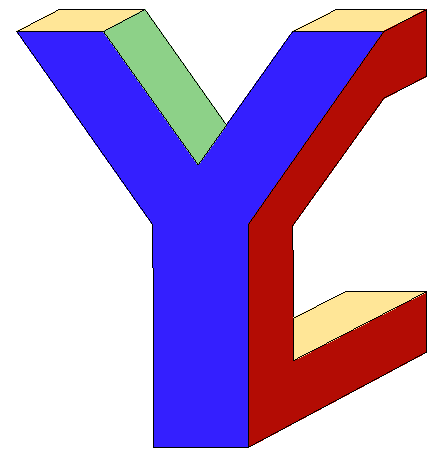
\includegraphics[height=1.5cm]{pictures/YC_logo.pdf}
    \end{center}
    &
    \begin{center}
      
\includegraphics[height=1.5cm]{pictures/SPbGU_Logo.png}
    \end{center}
  \end{tabular}
  \titlepage
\end{frame}
}


\begin{frame}[fragile]
 \frametitle{Мотивация}
\begin{center}
    $R \subset CF \subset Conj \subseteq Bool$
\end{center}
\begin{itemize}
    \item Кроме всем известной иерархии Хомского, есть довольно много классов формальных языков
    \item И не все они имеют свою лемму о накачке
    \item В последнее время все чаще прибегают к смежным дисциплинам для исследования языков
    \item Мы предлагаем построить группу по языку, чтобы в дальнейшем можно было применять аппарат теории групп для исследований
\end{itemize}
\end{frame}

\begin{frame}[fragile]{Связь с теорией групп}
        Пусть $\Sigma$ --- конечный алфавит, тогда
    \begin{itemize}
        \item $\Sigma^+$ --- свободная полугруппа
        \item $\Sigma^*$ --- свободный моноид
        \item $(\Sigma \cup \Sigma^{-1})^*$ --- свободная группа
    \end{itemize}
    \pause
        $G = \langle A~|~R \rangle$ --- представление группы
    \begin{itemize}
        \item $G = \langle a, b~|~a^3, b^2, (ab)^2 \rangle = \{\epsilon, a, a^2, b, ab, a^2b\} = S_3$
        \item $G = \langle a~|~a^5\rangle = C_5$
        \item $G = \langle a, b~|~aba^{-1}b^{-1} \rangle$
    \end{itemize}
\end{frame}

\begin{frame}[fragile]{Проблема слов}
    \begin{columns}[onlytextwidth,T]
        \column{\dimexpr\linewidth-60mm-5mm}
        $G = \langle A~|~R \rangle$, $\Sigma = A \cup A^{-1}$
        
        $\phi : \Sigma^* \to G$
        
        $W(G) = \phi^{-1}(1)$
        \newline
        \newline
        \begin{itemize}
            \item $W(G)$ -- регулярна $\iff G$ -- конечна (Anisimov)
            \item $W(G)$ -- контекстно-свободна $\iff \exists H < G$ -- конечного идекса (Muller–Schupp)
        \end{itemize}
        
        \column{60mm}
        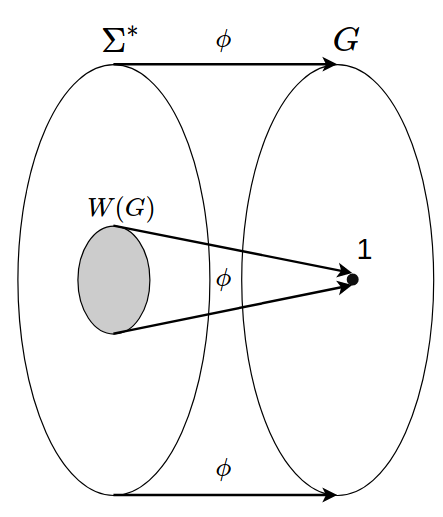
\includegraphics[width=60mm]{pictures/3.png}
    \end{columns}
\end{frame}

\begin{frame}[fragile]{Цель и задачи}
\textbf{Цель:} Создать инструмент, с помощью которого можно будет смотреть на формальные языки как на группы
\newline
\newline
\textbf{Задачи:}
    \begin{enumerate}
        \item Реализовать алгоритм построения группы по машине Тьюринга
        \item Доказать корректность алгоритма
    \end{enumerate}
\end{frame}

\begin{frame}[fragile]{Построение группы (0)}
\begin{center}
    Mark V. Sapir, Jean-Camille Birget and Eliyahu Rips "Isoperimetric and Isodiametric Functions of Groups" (2002)
    \end{center}
    \begin{block}{Теорема 1}
		Пусть $L \subseteq \Sigma^+$ язык, принимаемый машиной Тьюринга $M$,
    тогда существует конечно представленная группа $G(M)=\langle A~|~R \rangle$
    и инъективное отображение $K: \Sigma^+ \to (A \cup A^{-1})^+$ такое что:
    $u \in L \iff K(u)=1_G$
	\end{block}
\end{frame}

\begin{frame}[fragile]{Построение группы (1)}
\begin{block}{Теорема 2}
Для любой машины Тьюринга M существует симметричная машина Тьюринга M' со следующими свойствами:
    \begin{itemize}
        \item Распознает тот же язык, что и M
        \item Каждая команда действует только на одной ленте
        \item Добавляется лента, алфавитом которой являются команды
    \end{itemize}
\end{block}
\pause
\begin{block}{Теорема 3}
Для любой машины Тьюринга M', удовлетворяющей теореме 2, существует S-машина, которая симулирует M'
\end{block}
\pause
\begin{block}{Теорема 4}
Для любой S-машины, удовлетворяющей теореме 3, существует соответствующая конечно представленная группа
\end{block}
\end{frame}

\begin{frame}[fragile]{Построение группы (2)}
\begin{figure}[H]
  \centering
  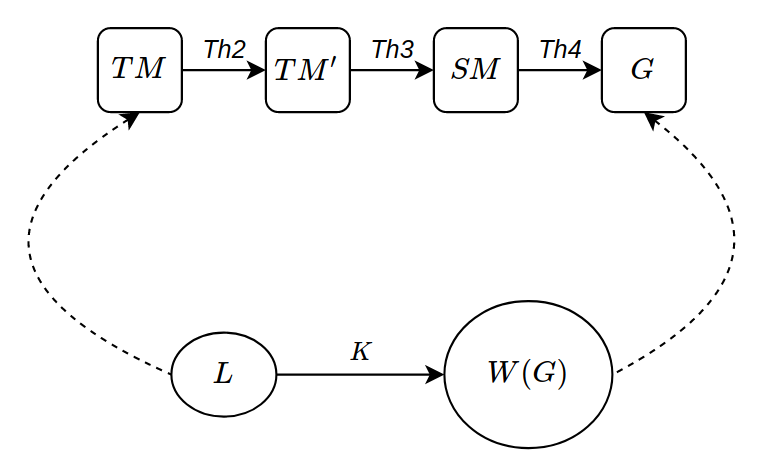
\includegraphics[width=120mm]{pictures/2.png}
 \end{figure}
\end{frame}

\begin{frame}[fragile]{Результаты и дальнейшие действия}
    \begin{itemize}
        \item Реализован алгоритм
        \item Проведен ряд экспериментов
        \item Найдена более свежая статья
        \item Рассматривается возможность формальной верификации алгоритма
    \end{itemize}
\end{frame}

\end{document}
